%!TEX program = xelatex
\documentclass{beamer}
%\documentclass[aspectratio=169]{beamer} %如果需要16:9
\usepackage{ctex}
\usepackage{times}
\usepackage{multicol}
\usepackage{multirow}
\usetheme{Warsaw}
\usepackage{tikz}
\usetikzlibrary{arrows,shapes,chains}
\usepackage[super,square]{natbib}
%\usecolortheme{beaver}     % use white-grey colour style
%\beamersetaveragebackground{black!10}
% This is only inserted into the PDF information catalog. Can be left out.
\subject{presentation}
\keywords{example}
\useinnertheme{circles}%{rectangles}
\setbeamertemplate{itemize item}{$\circledast$}%{\checkmark}

%% ======================================================
%%     preamble
%% ======================================================
\title{大学生创业平台的开发与系统优化策略研究}
\author{武斌}
\institute
{
  电子系~中国海洋大学
  \and
   Department electronic engineering \\
  Ocean University Of China
}
\date{\today}

\logo{
\includegraphics[height=0.09\textwidth]{./logo/Ocean_University_of_China.png}}


%% ======================================================
\begin{document}

%% ++++++++++++++++++++++++++++++++++++++++++++++++++++++
%% title page
%% ++++++++++++++++++++++++++++++++++++++++++++++++++++++
\begin{frame}
  \titlepage
\end{frame}

%% ++++++++++++++++++++++++++++++++++++++++++++++++++++++
%%     Table of Contents
%% ++++++++++++++++++++++++++++++++++++++++++++++++++++++
%\begin{frame}
    %\frametitle{Contents}
    %\tableofcontents
    %% 显示1-4section,不显示subsection
    %\tableofcontents[hidesubsections,sections={<1-4>}]
%\end{frame}

%% ++++++++++++++++++++++++++++++++++++++++++++++++++++++
%%     目录
%% ++++++++++++++++++++++++++++++++++++++++++++++++++++++
%\section{概述}
\begin{frame}
  \frametitle{概述}
  \begin{enumerate}
    \item<1-> 选题背景
    \item<1-> 研究内容
    \item<1-> 研究方案
    \item<1-> 进展情况
  \end{enumerate}
\end{frame}


%% ++++++++++++++++++++++++++++++++++++++++++++++++++++++
%%      正文
%% ++++++++++++++++++++++++++++++++++++++++++++++++++++++
%% ++++++++++++++++++++++++++++++++++++++++++++++++++++++
%%      选题背景
%% ++++++++++++++++++++++++++++++++++++++++++++++++++++++
%\section{选题来源和背景分析 }
%\subsection{系统结构}
\begin{frame}
  \frametitle{选题背景}
  \begin{block}{课题来源}
  	\begin{itemize}
  		\item 创业过程中负责创游记平台的系统开发、维护和WEB开发
  		\item 海信实习过程中参与小微系统开发、环境部署与优化的工作
  	\end{itemize}
  \end{block}
  \pause %分页显示
  \begin{block}{选题依据和背景情况}
  	\begin{itemize}
  		\item \cite{chuangye1}进行创业实践的大学生不断增多,开发一个大学生创新创业的平台,提供创业指导、成果展示、投融资推荐和就业机会的推荐等服务,针对平台用户的创业行为进行分析与研究
      \item WEB产品不断增加,很多产品在系统优化方面做的比较少,无论是系统的持续集成还是系统负载的平衡以及性能的优化等方面,本课题将以平台为案例进行系统优化等方面的研究
  	\end{itemize}
  \end{block}
\end{frame}

\begin{frame}
  \frametitle{选题背景}
  \begin{block}{课题研究目的}
  	\begin{itemize}
  		\item 基于WEB技术开发一款服务于大学生创新创业的网络平台
  		\item 研究系统开发过程中的代码、持续集成、负载等方面的优化策略
  	\end{itemize}
  \end{block}
  \pause
  \begin{block}{理论意义和研究价值}
  	\begin{itemize}
  		\item 从平台功能而言,希望可以帮助大学生进行创新创业方面的尝试和实践,帮助投资机构寻找具有商业价值的创业项目或者创业者
  		\item 从研究角度而言,希望可以通过开发和使用更好的技术来提升系统在使用过程中的代码、部署、测试以及负载等方面的性能,研究一体化的优化策略
  	\end{itemize}
  \end{block}
\end{frame}

%% ++++++++++++++++++++++++++++++++++++++++++++++++++++++
%%      研究内容
%% ++++++++++++++++++++++++++++++++++++++++++++++++++++++
\begin{frame}
  \frametitle{研究内容}
  \begin{enumerate}
    \item<1-> 创游记平台的开发
    \item<1-> 系统优化策略研究
  \end{enumerate}
\end{frame}

\begin{frame}
  \frametitle{创游记平台的开发}
  \begin{figure}
  \centering
    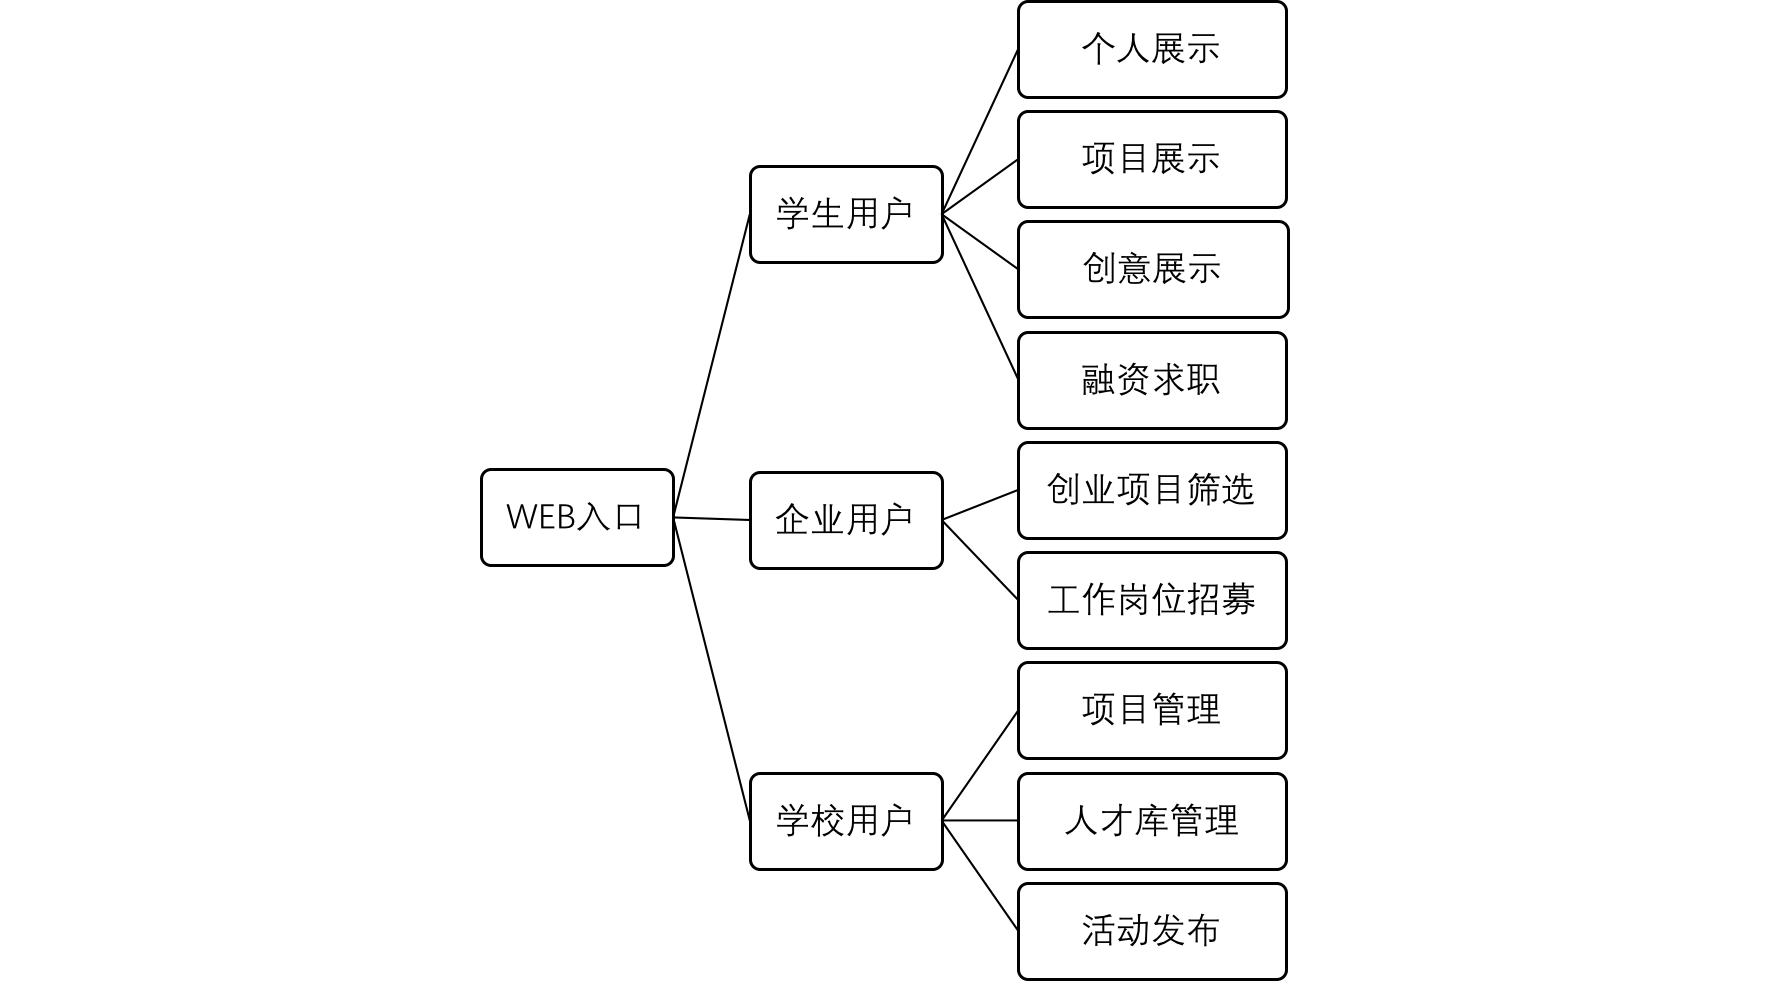
\includegraphics[height=6cm]{./img/web_frame.png}
    \caption{平台功能}
    \label{fig:visual}
  \end{figure}
\end{frame}

\begin{frame}
  \frametitle{创游记平台的开发}
  \begin{columns}
    \begin{column}{0.50\textwidth}
      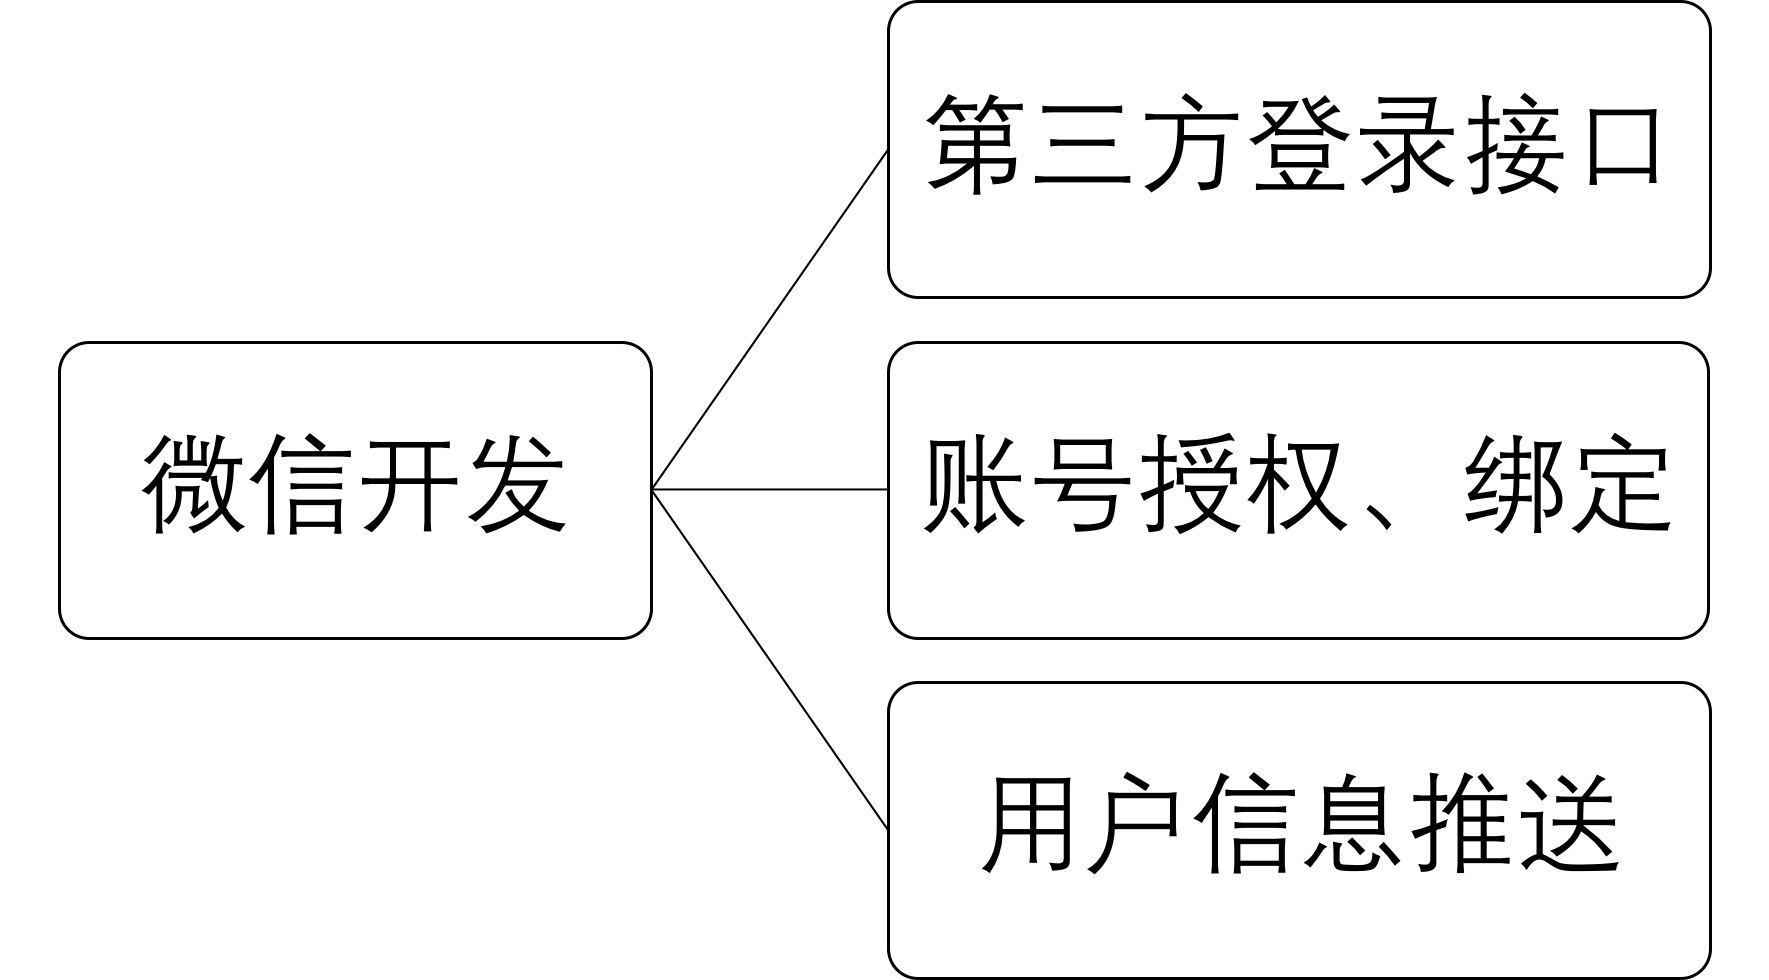
\includegraphics[width=\textwidth]{./img/web_weixin.png}
    \end{column}
    \begin{column}{0.50\textwidth}
      \begin{block}{开发目标}
        \begin{enumerate}
          \item 针对不同用户完成不同功能模块的开发
          \item 实现微信端的浏览、访问、授权
          \item 实现针对定向用户的个性化推荐
        \end{enumerate}
      \end{block}
    \end{column}
  \end{columns}
\end{frame}

\begin{frame}
\frametitle{针对平台的优化策略研究}
  \begin{block}{代码优化 }
  	\begin{itemize}
  		\item 整合平台开发过程中过多代码复用的功能到公共函数库,实现模块化的开发
  		\item 将特定功能写成系统插件或者框架,提升代码运行效率
  	\end{itemize}
  \end{block}
  \begin{block}{推荐系统开发}
  	\begin{itemize}
  		\item 探索基于平台用户数据的推荐系统开发,实现学生用户的融资求职机会推荐和企业用户的创业项目推荐
  	\end{itemize}
  \end{block}
\end{frame}

\begin{frame}
  \frametitle{针对系统的优化策略研究}
  \begin{block}{持续集成环境构建 }
    \begin{itemize}
      \item 探索在本地环境搭建一个持续集成环境,实现一个自动构建过程,包括自动编译、分发、部署和测试等功能
    \end{itemize}
  \end{block}
  \pause %分页显示
  \begin{block}{系统缓存开发}
  	\begin{itemize}
  		\item 探索系统缓存对于WEB系统性能的影响
      \item 基于本系统研究系统的缓存机制和策略
      \item 基于本系统进行缓存机制的开发和性能测试
  	\end{itemize}
  \end{block}
  \pause %分页显示
  \begin{block}{搜索优化 }
  	\begin{itemize}
  		\item 研究在保证搜索的实时、稳定、可靠和快速基础上,降低系统负载的方式
      \item 探索基于分布式搜索的系统接口开发和性能测试
  	\end{itemize}
  \end{block}
\end{frame}

%% ++++++++++++++++++++++++++++++++++++++++++++++++++++++
%%      研究方案
%% ++++++++++++++++++++++++++++++++++++++++++++++++++++++
\begin{frame}
  \frametitle{研究方案}
  \begin{enumerate}
      \item<1-> 创游记平台的开发
      \item<1-> 平台代码优化
      \item<1-> 推荐系统研究与开发
      \item<1-> 自动化测试部署方案研究
      \item<1-> 系统缓存和优化方案研究
  \end{enumerate}
\end{frame}

\begin{frame}
  \frametitle{创游记平台的开发}
  \begin{block}{基本环境搭建 }
	  \begin{itemize}
		  \item 搭建基于Linux+Apache+MySQL+PHP/Python的WEB开发环境
      \item 搭建本地的代码版本控制工具GitLab
	  \end{itemize}
  \end{block}
\end{frame}

\begin{frame}
  \frametitle{创游记平台的开发}
  \begin{figure}
    \centering
      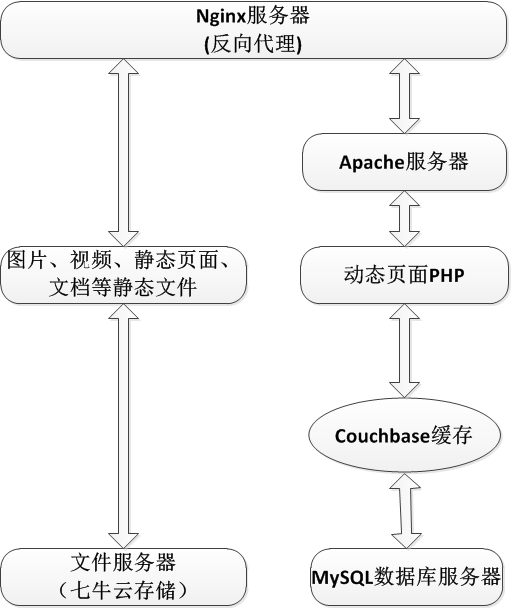
\includegraphics[height=6cm]{./img/web_frame2.png}
    \caption{平台基本框架}
    \label{fig:visual}
  \end{figure}
\end{frame}

\begin{frame}
  \frametitle{创游记平台的开发}
  \begin{columns}
    \begin{column}{0.40\textwidth}
      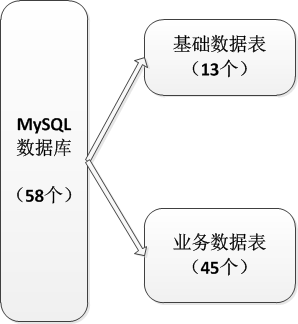
\includegraphics[width=\textwidth]{./img/mysql.png}
    \end{column}
    \begin{column}{0.60\textwidth}
      \begin{block}{数据表设计和维护}
        \begin{itemize}
          \item 基础数据表主要包括系统的基本环境配置、插件配置、文档模型配置等
          \item 业务数据表主要包含用户、活动、项目、创意等数据
        \end{itemize}
      \end{block}
    \end{column}
  \end{columns}
\end{frame}

\begin{frame}
  \frametitle{创游记平台的开发}
  \begin{block}{平台代码优化}
    \begin{itemize}
      \item 模块化表单功能开发,通过开发FormBuilder和ListBuilder两个模块以及在数据库中配置界面字典和物理字典,实现表单的统一配置和显示,避免了在每一个页面都复写form的复杂操作
      \item 开发JS提交插件AJAXPost和JAJXGet实现数据提交和获取,避免在每一个前端页面和后台控制器中都配置数据变量和返回格式的问题
      \item 开发JS上传插件Uploader,实现文件的上传、图片的上传和修改等功能以及七牛云存储的保存
    \end{itemize}
  \end{block}
\end{frame}

\begin{frame}
\frametitle{\cite{crab1}推荐系统研究与开发}
  \begin{block}{常用的推荐系统算法}
    \begin{enumerate}
      \item 基于内容的推荐-推荐和用户过去喜欢项的内容相似的项
      \item 协同过滤推荐-通过在用户的一系列行为中寻找特定模式来产生用户特殊推荐
      \item 混合推荐-综合以上两种算法的优点同时抵消各自的缺点
      \item 高级非传统的推荐-深度学习、上下文感知推荐等
    \end{enumerate}
  \end{block}
  \pause
  \begin{block}{本课题使用的推荐算法和框架}
    \begin{itemize}
      \item 本课题主要使用协同过滤推荐算法中的基于用户的协同过滤算法
      \item \cite{crab2}本课题使用的框架是基于Python的Crab推荐系统引擎
    \end{itemize}
  \end{block}
\end{frame}

\begin{frame}
\frametitle{推荐系统研究与开发}
  \begin{block}{协同过滤推荐算法(Collaborative Filtering Recommendation)}
    \begin{itemize}
      \item 基于用户的协同过滤(User-Based CF)\\
      找到和目标用户兴趣相似的用户集合,然后给目标用户推荐这个集合的用户喜欢的物品
      \item 基于物品的协同过滤(Item-Based CF)\\
      给目标用户推荐与他喜欢的物品相似度较高高的物品\\
    \end{itemize}
  \end{block}
  \pause
  \begin{block}{选择基于用户的协同过滤的原因}
    \begin{itemize}
      \item 适合用户较少的场合,否则用户相似度矩阵计算代价很大
      \item 适合时效性较强,用户个性化兴趣不太明显的领域
    \end{itemize}
  \end{block}
\end{frame}

\begin{frame}
\frametitle{基于用户的协同过滤算法的主要公式和步骤}
  \begin{itemize}
    \item \cite{crab3} 基于用户的协同过滤的关键在于计算用户与用户之间的兴趣相似度,主要使用余弦相似度来计算:\\
    \begin{displaymath}
    \omega_{\mu\nu} = \frac{|N(\mu) \cap N(\nu)|}{\sqrt{|N(\mu) \parallel N(\nu)|}}
    \end{displaymath}
    $\omega_{\mu\nu}$代表用户 $\mu$ 与 $ \nu $ 之间的兴趣相似度,$ {N(\mu)} $ 表示用户 $ \mu $ 曾经喜欢过的物品集合, $ {N(\nu)} $ 表示用户 $ \nu $ 曾经喜欢过的物品集合
    \item 根据上述描述,可以有如下算法步骤
      \begin{enumerate}
        \item 建立物品-用户的倒排表(Inverted Index)
        \item 计算用户与用户之间的共享矩阵 $C[\mu][\nu]$,表示用户$\mu$与$\nu$喜欢相同物品的个数
        \item 计算用户与用户之间的相似度矩阵 $\omega[\mu][\nu]$,根据上述相似度计算公式计算
        \item 用上面的相似度矩阵来给用户推荐和他兴趣相似的用户喜欢的物品
      \end{enumerate}
  \end{itemize}
\end{frame}

\begin{frame}
\frametitle{推荐系统研究与开发}
  \begin{block}{Crab推荐系统引擎}
    \begin{itemize}
      \item Crab是基于Python开发的开源推荐软件,其中实现的方法有item和user的协同过滤,其他的一些算法在开发中
      \item 基于scikit-learn库,scikit-learn库是Python下的一个机器学习库,建立在NumPy,SciPy和matplotlib模块之上,可以实现很多机器学习的算法,为用户提供各种机器学习算法接口,让用户简单、高效地进行数据挖掘和数据分析
    \end{itemize}
  \end{block}
  \begin{figure}
    \centering
      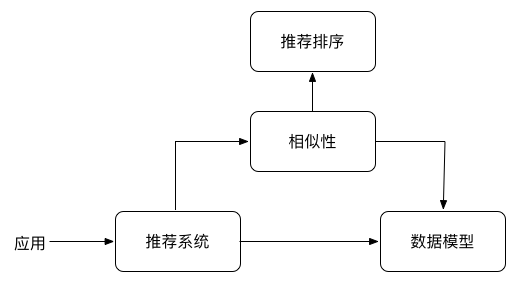
\includegraphics[height=3cm]{./img/crab.png}
    \caption{crab框架}
    \label{fig:visual}
  \end{figure}
\end{frame}


\begin{frame}
\frametitle{持续集成方案研究}
  \begin{block}{关于持续集成}
    持续集成是一种软件开发实践,通过频繁地(一天多次)将代码集成到主干。每次集成都通过自动化的构建(包括编译,发布,自动化测试)来验证,从而尽早地发现集成错误\cite{jenkins1}。
  \end{block}
  \pause
  \begin{block}{持续集成的好处\cite{jenkins2}}
    \begin{enumerate}
      \item 快速发现错误。每完成一点更新,就集成到主干,可以快速发现错误,定位错误也比较容易。
      \item 防止分支大幅偏离主干。如果不是经常集成,主干又在不断更新,会导致以后集成的难度变大,甚至难以集成。
    \end{enumerate}
  \end{block}
  \pause
  \begin{block}{持续集成的目的}
    让产品可以快速迭代,同时还能保持高质量。它的核心措施是,代码集成到主干之前,必须通过自动化测试。只要有一个测试用例失败,就不能集成。
  \end{block}
\end{frame}

\begin{frame}
\frametitle{持续集成方案研究}
  \begin{block}{本课题搭建持续集成的目的和研究}
    \begin{itemize}
      \item 在使用持续集成方案之前,系统的部署流程是直接将代码通过GitLab的钩子(hook)将代码同步到服务器端的WEB目录下,没有进行自动化的构建、测试和部署。
    \end{itemize} 
  \end{block}
  \begin{figure}
    \centering
      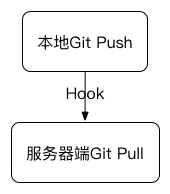
\includegraphics[height=5cm]{./img/jenkins1.png}
    \caption{原部署流程}
    \label{fig:visual}
  \end{figure}
\end{frame}

\begin{frame}
\frametitle{持续集成方案研究}
  \begin{block}{本课题搭建持续集成的目的和研究}
    \begin{itemize}
      \item 使用持续集成方案之后,通过GitLab的钩子(hook)触发系统的持续集成工具,对代码进行合并、构建、测试和部署,出现重大问题时可以回滚。
    \end{itemize} 
  \end{block}
  \begin{figure}
    \centering
      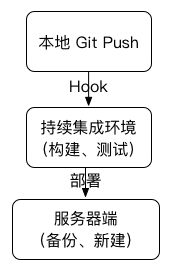
\includegraphics[height=5cm]{./img/jenkins2.png}
    \caption{现部署流程}
    \label{fig:visual}
  \end{figure}
\end{frame}

\begin{frame}
\frametitle{持续集成方案研究}
  \begin{block}{集成环境的搭建和配置}
    \begin{itemize}
      \item 本地搭建Jenkins持续集成服务器,并且安装针对PHP的构建、测试插件
      \item 针对关键功能开发自动化测试脚本,在Jenkins集成时调用 
      \item 开发Hook触发脚本和持续部署脚本,实现服务器端的的代码更新和文件备份 
    \end{itemize} 
  \end{block}
  \begin{block}{Jenkins简介}
    \begin{itemize}
      \item Jenkins 是一个开源项目,提供一种易于使用的持续集成系统,使开发者从繁杂的集成中解脱出来,专注于更为重要的业务逻辑实现上。
      \item 同时 Jenkins 能实时监控集成中存在的错误,提供详细的日志文件和提醒功能,还能用图表的形式形象地展示项目构建的趋势和稳定性。
    \end{itemize} 
  \end{block}
\end{frame}


\begin{frame}
\frametitle{系统缓存和优化方案研究}
  \begin{itemize}
    \item 系统之前版本和现在版本使用的缓存机制对比
  \end{itemize} 
  \begin{columns}
    \begin{column}{0.50\textwidth}
      \begin{figure}
        \centering
          
\includegraphics[height=6cm]{./img/couchbase1.png}
        \caption{之前数据操作模型}
        \label{fig:visual}
      \end{figure}
    \end{column}
    \begin{column}{0.50\textwidth}
      \begin{figure}
        \centering
          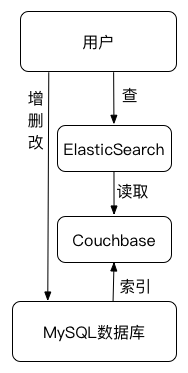
\includegraphics[height=6cm]{./img/couchbase2.png}
        \caption{当前数据操作模型}
        \label{fig:visual}
      \end{figure}
    \end{column}
  \end{columns}
\end{frame}

\begin{frame}
\frametitle{系统缓存和优化方案研究}
  \begin{block}{Couchbase缓存\cite{couchbase1} }
    \begin{itemize}
      \item Couchbase是一个具有高性能、可扩展性和可用性强的NoSQL数据库引擎
      \item 使用Couchbase将系统的业务数据在系统启动时加载到缓存中,有效降低系统的负载并加快数据读取速度 
      \item 使用Couchbase缓存机制可以降低系统的丢包率,增强系统的稳定性
    \end{itemize} 
  \end{block}
  \begin{block}{ElasticSearch搜索引擎\cite{elasticsearch1} }
    \begin{itemize}
      \item Elasticsearch是一个基于Apache Lucene(TM)的开源搜索引擎
      \item 实时分析搜索引擎,每个字段都被索引并可被搜索
      \item RESTful 搜索引擎,能够达到搜索实时、稳定、可靠和快速,支持通过HTTP请求,使用JSON进行数据索引\cite{elasticsearch2}
    \end{itemize} 
  \end{block}
\end{frame}

\begin{frame}
\frametitle{系统缓存和优化方案研究}
  \begin{block}{七牛云存储}
    \begin{itemize}
      \item 将平台的图片和视频等媒体数据上传到七牛云存储
      \item 通过七牛的CND加速加快系统图片和视频的加载速度
    \end{itemize} 
  \end{block}
  \begin{block}{WEB缓存的意义和作用}
    \begin{itemize}
      \item 减少网络带宽消耗
      \item 降低服务器压力
      \item 减少网络延迟,加快页面打开速度
    \end{itemize} 
  \end{block}
\end{frame}
%% ++++++++++++++++++++++++++++++++++++++++++++++++++++++
%%      进展情况
%% ++++++++++++++++++++++++++++++++++++++++++++++++++++++
\begin{frame}
\frametitle{进展情况}
  \begin{block}{已完成 }
	\begin{itemize}
		\item 平台功能开发
		\item Jenkins自动化测试、部署工具的配置和部署脚本开发
        		\item Couchbase缓存机制的开发
		\item ElasticSearch分布式全文搜索引擎的部署和测试
	\end{itemize}
  \end{block}
  \pause %分页显示
  \begin{block}{进行中}
	\begin{itemize}
    \item 缓存和搜索接口的开发
    \item 推荐系统的开发
	\end{itemize}
  \end{block}
\end{frame}

%% ++++++++++++++++++++++++++++++++++++++++++++++++++++++
%%      Last Page
%% ++++++++++++++++++++++++++++++++++++++++++++++++++++++
% \begin{frame}
% \frametitle{大学生创业平台的开发与系统优化策略研究}
%   谢谢各位老师的聆听!
% \end{frame}

%% ++++++++++++++++++++++++++++++++++++++++++++++++++++++
%%      Reference Page
%% ++++++++++++++++++++++++++++++++++++++++++++++++++++++
\begin{frame}[allowframebreaks]{References}
  \scriptsize
  \bibliographystyle{plain}
  \bibliography{myRefs}
\end{frame}

\end{document}
%% ======================================================
